\chapter{OPTIMIZACIÓN DEL FILTRO DE KALMAN EXTENDIDO MEDIANTE ESTADO AUMENTADO}
\label{ch:optimizacion_kalman}

En este capítulo se detalla la reformulación matemática del Filtro de Kalman Extendido (EKF) empleado para el seguimiento de la etiqueta UWB. Durante las pruebas iniciales, el EKF convencional mostró un desempeño limitado frente a los errores sistemáticos propios de la tecnología UWB, tales como el sesgo por ancla, las trayectorias NLOS y las reflexiones multipath. Por ello, se rediseñó el estimador matemático pasando de un modelo de seguimiento de posición pura a un modelo de \textit{estado aumentado} con estimación concurrente de sesgos, complementado con una fase de actualización iterada (IEKF).

\section{Planteamiento del Problema en el Modelo Original}
El modelo original del EKF basaba su vector de estado únicamente en las coordenadas espaciales bidimensionales de la etiqueta:
\begin{equation}
    x_k = \begin{bmatrix} p_{x,k} \\ p_{y,k} \end{bmatrix}
\end{equation}

Bajo este esquema, la medición de distancia hacia la ancla $i$ se modelaba idealmente como la distancia euclidiana más un ruido blanco gaussiano $v_{i,k}$:
\begin{equation}
    z_{i,k} = \sqrt{(p_{x,k} - a_{i,x})^2 + (p_{y,k} - a_{i,y})^2} + v_{i,k}
\end{equation}
donde $a_i = [a_{i,x}, a_{i,y}]^T$ representa las coordenadas conocidas del ancla $i$.

El inconveniente fundamental de esta formulación radica en la naturaleza empírica de las mediciones UWB en entornos interiores. Las distancias medidas suelen presentar un sesgo aditivo sistemático $\beta_i$ proveniente de retardos en el hardware, calibración imperfecta de la antena o condiciones de propagación. Al no incluir este término en el modelo matemático, el residual o innovación del filtro $\nu_k = z_k - h(x_k^-)$ se ve forzado a ser absorbido enteramente por el vector de estado espacial. En consecuencia, el filtro proyecta erróneamente los sesgos de medición como desviaciones de posicionamiento físico, deformando severamente la trayectoria estimada.

\section{Reformulación Matemática: EKF con Sesgo Dual Dependiente del Rango}
Para mitigar el error de especificación del modelo original y abordar los fenómenos de propagación complejos de las señales UWB, se procedió a aumentar el vector de estado. A diferencia de un modelo de sesgo simple, las mediciones UWB exhiben perturbaciones que dependen de la distancia entre la etiqueta y la ancla (efectos de campo cercano, retardos asimétricos de antena). Por ende, se introdujo un modelo de \textit{sesgo dual} que incluye un sesgo constante a larga distancia ($b_{far}$) y un sesgo variable que decae exponencialmente en distancias cortas ($b_{near}$).

El nuevo estado $x_k \in \mathbb{R}^{10}$ se define como:
\begin{equation}
    x_k = \begin{bmatrix} p_{x,k} \\ p_{y,k} \\ b_{far,1,k} \\ \vdots \\ b_{far,4,k} \\ b_{near,1,k} \\ \vdots \\ b_{near,4,k} \end{bmatrix}
\end{equation}

La matriz de transición de estado se establece como la matriz identidad ($F = I_{10}$), asumiendo una dinámica estática entre las ventanas de muestreo, donde tanto la posición como los sesgos evolucionan gobernados por procesos de ruido aleatorio. La matriz de covarianza del ruido de proceso $Q$ se configura para otorgar flexibilidad a los cambios de posición y una variación conservadora diferenciada a los sesgos:
\begin{equation}
    Q = \operatorname{diag}(q_{pos}, q_{pos}, q_{far}, \dots, q_{far}, q_{near}, \dots, q_{near})
\end{equation}

El modelo de medida modificado incorpora de forma explícita este comportamiento no lineal:
\begin{equation}
    z_{i,k} = \lVert p_k - a_i \rVert + b_{far,i,k} + b_{near,i,k} e^{-\lambda \lVert p_k - a_i \rVert} + v_{i,k}
\end{equation}
donde $\lambda$ representa una constante empírica de decaimiento espacial (típicamente $\lambda = 0.15$).

La inclusión de la no linealidad altera fundamentalmente la matriz Jacobiana $H_k$, expandiéndola a unas dimensiones de $4 \times 10$. El gradiente espacial ya no es puramente geométrico, sino que se ve modulado por el efecto del sesgo cercano. Para la ancla $i$, las derivadas parciales correspondientes a la posición y a sus respectivos sesgos se evalúan como:
\begin{align}
    \frac{\partial z_{i,k}}{\partial p_{x,k}} &= \frac{p_{x,k} - a_{i,x}}{r_i} \left( 1 - \lambda b_{near,i,k} e^{-\lambda r_i} \right) \\
    \frac{\partial z_{i,k}}{\partial p_{y,k}} &= \frac{p_{y,k} - a_{i,y}}{r_i} \left( 1 - \lambda b_{near,i,k} e^{-\lambda r_i} \right) \\
    \frac{\partial z_{i,k}}{\partial b_{far,i,k}} &= 1 \\
    \frac{\partial z_{i,k}}{\partial b_{near,i,k}} &= e^{-\lambda r_i}
\end{align}
donde $r_i = \lVert p_k - a_i \rVert$. 

Esta formulación es estructuralmente superior debido a que la ganancia de Kalman puede ahora separar, de manera probabilística, la innovación de la medición en múltiples flujos de compensación independientes: corrigiendo la geometría espacial (movimiento físico), absorbiendo el error sistemático global del hardware (sesgo $far$), y mitigando las distorsiones complejas que ocurren cuando la etiqueta se acerca a las anclas (sesgo $near$).

\section{Filtro de Kalman Extendido Iterado (IEKF)}
Debido a que la función de rango $h(x)$ ahora contiene no linealidades complejas, no solo originadas por la distancia geométrica pura $\lVert p - a_i \rVert$ sino por el término exponencial $e^{-\lambda \lVert p - a_i \rVert}$ del sesgo cercano, linealizarla una única vez alrededor del estado predicho $\hat{x}_k^-$ puede generar errores de truncamiento por series de Taylor muy significativos. Esto es crítico si la predicción inicial se encuentra alejada de la posición de referencia real. Para compensar esta deficiencia geométrica, la fase de corrección estándar se reemplazó por la arquitectura del EKF Iterado (IEKF). 

En el paradigma IEKF, las ecuaciones de actualización de estado, covarianza y el recálculo de la matriz Jacobiana $H_k$ se ejecutan cíclicamente dentro del mismo instante $k$ hasta cumplir un criterio de convergencia local estricto (por ejemplo, cambios residuales en la magnitud del vector de estado menores a una tolerancia de $10^{-9}$). Este mecanismo cíclico garantiza que la linealización final converja iterativamente hacia el gradiente más óptimo, constituyendo una aproximación sumamente robusta a la solución ideal del problema general de estimación por mínimos cuadrados no lineales.

\section{Validación Empírica del Filtro Optimizado}
La implementación en el software de la arquitectura de estado aumentado aunada al IEKF condujo a una reducción categórica de los márgenes de error de posicionamiento a través de todos los escenarios experimentales evaluados dentro del recinto cerrado. 

Como evidencia gráfica y cuantitativa, la Figura \ref{fig:comparativa_kalman} contrasta la precisión topológica obtenida mediante el EKF Original (Baseline) frente al modelo propuesto de EKF con Sesgo Dual No Lineal, procesando el banco de datos recolectado con el dispositivo localizado en la cadera del sujeto de prueba número 2.

\begin{figure}[H]
    \centering
    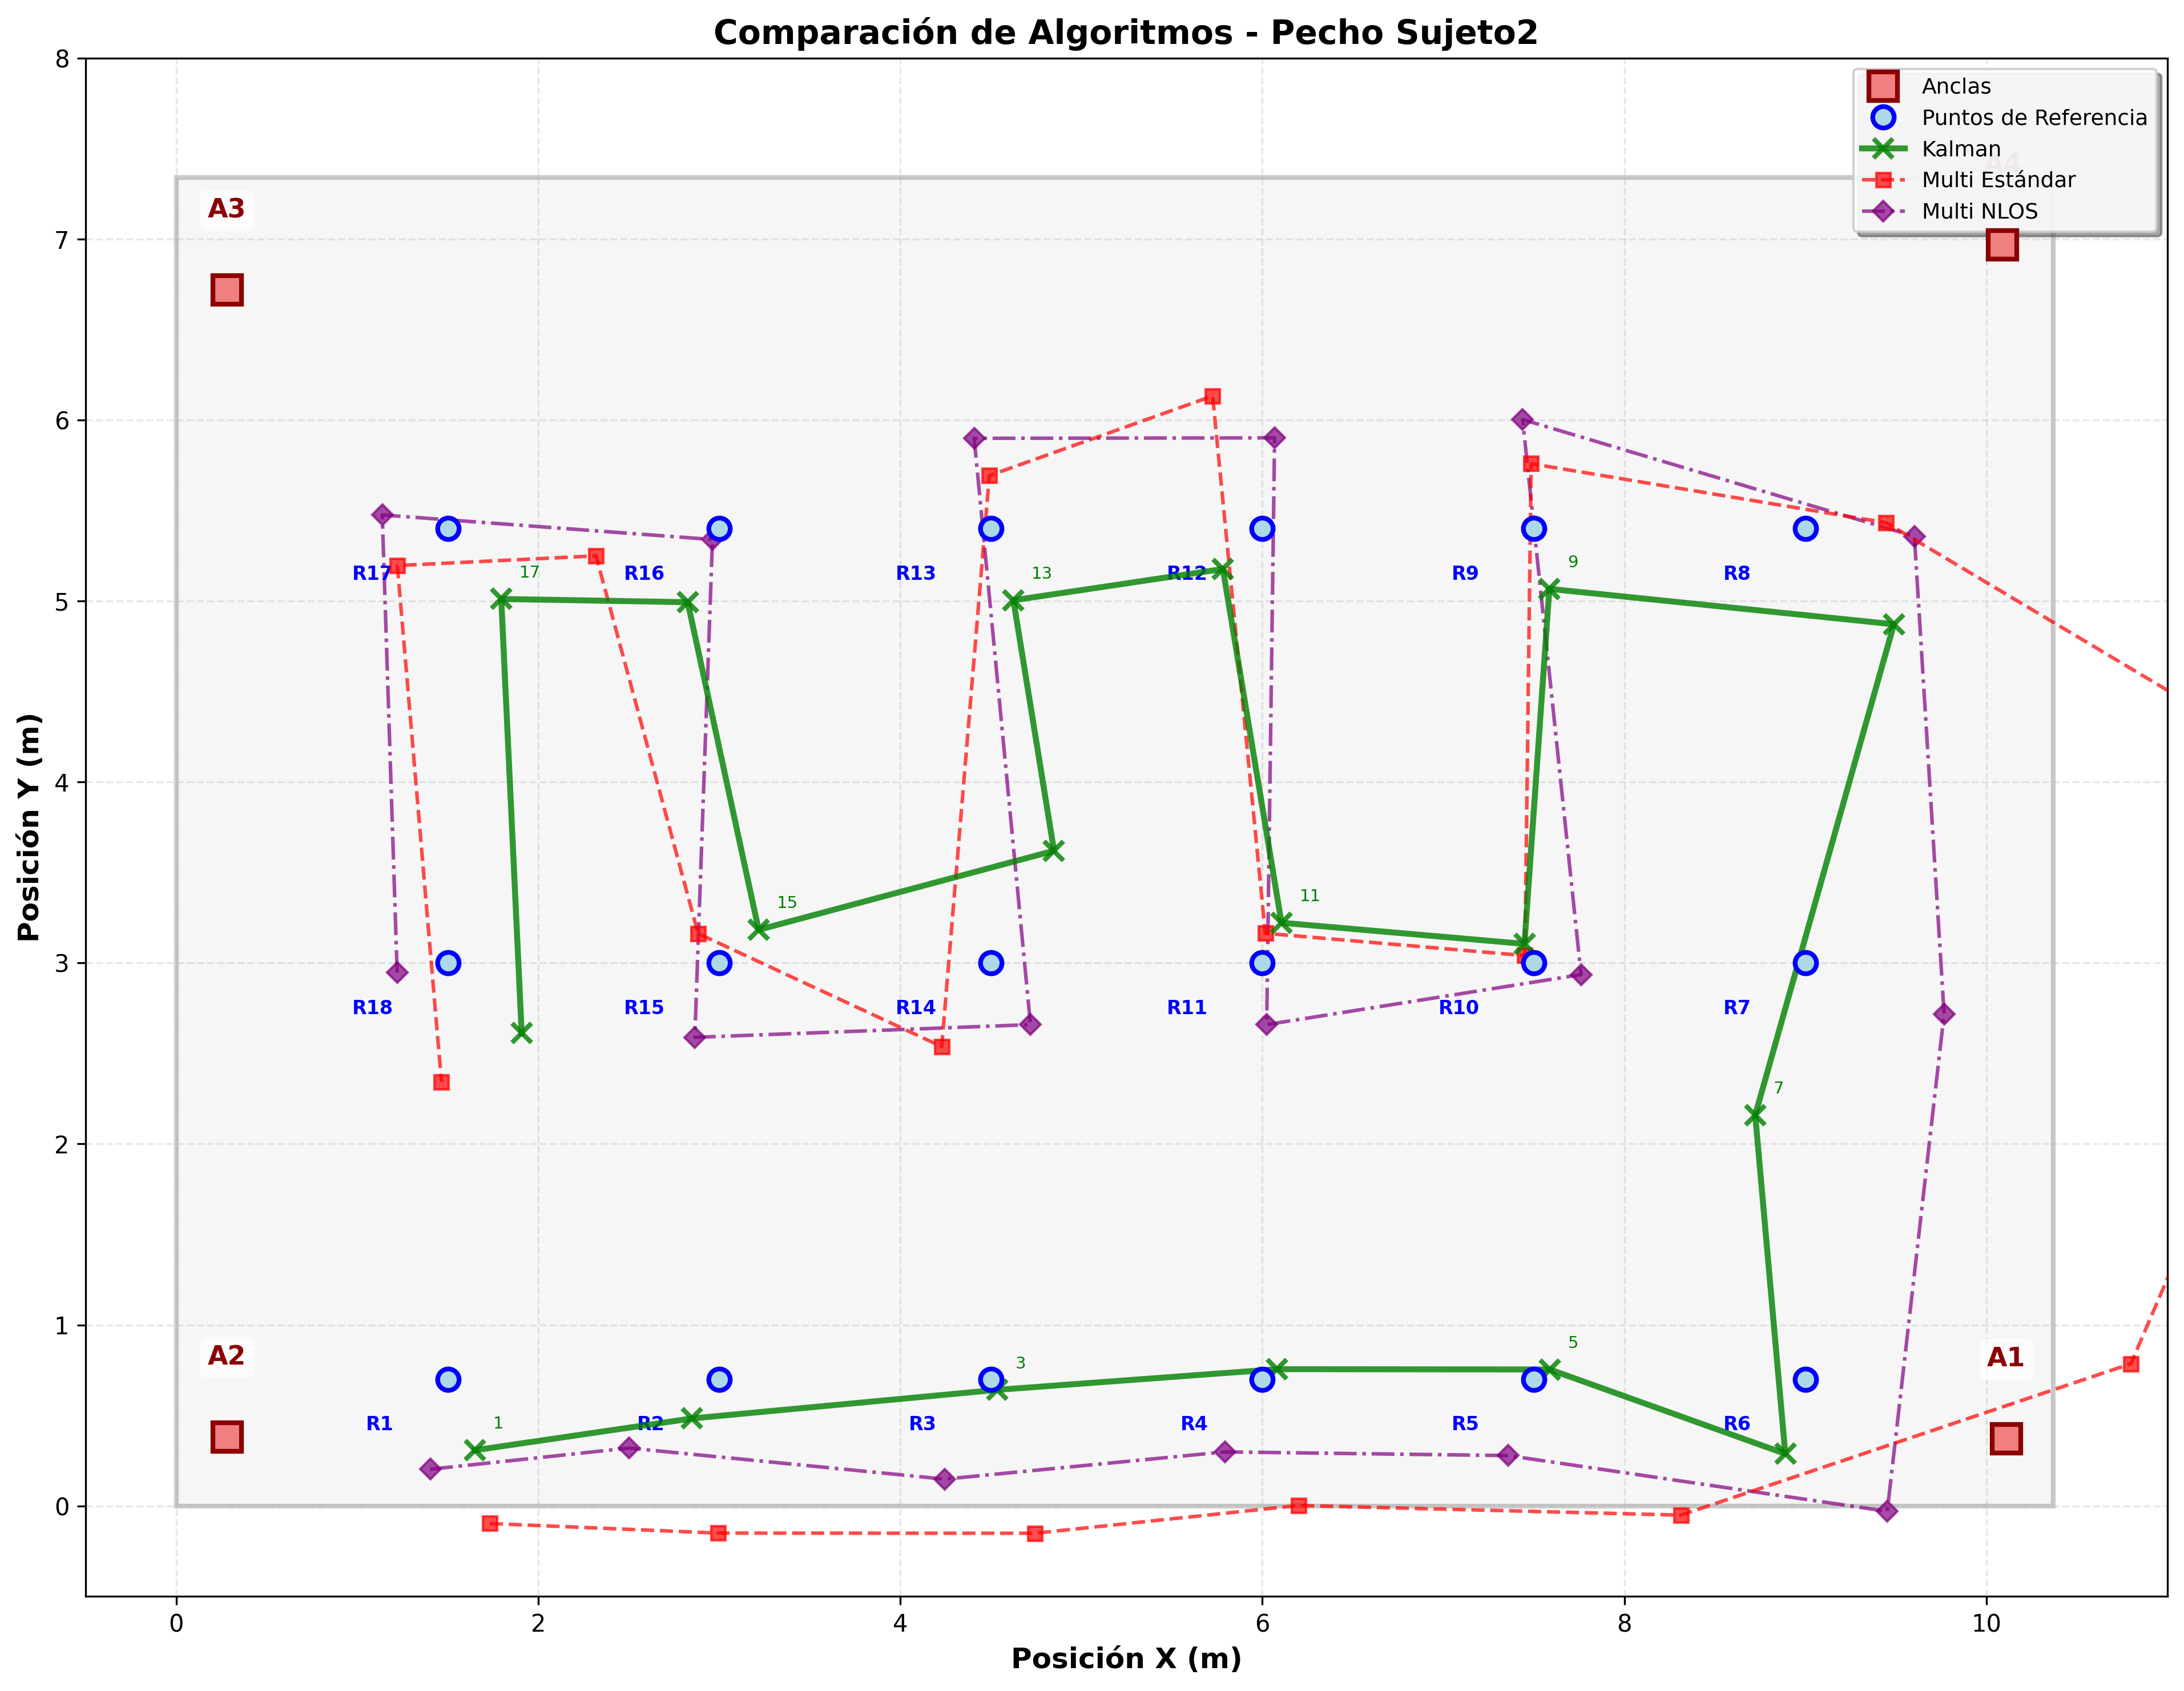
\includegraphics[width=\textwidth]{imagenes/mejora_kalman.png}
    \caption{Comparativa de estimación de trayectorias: EKF de posición pura vs. EKF con estado aumentado (sesgo dual no lineal). Escenario de prueba: sensor en la cadera del sujeto 2.}
    \label{fig:comparativa_kalman}
\end{figure}

El análisis de la Figura \ref{fig:comparativa_kalman} evidencia de manera indudable cómo la arquitectura EKF original (cuadrados rojos) presenta desviaciones sistemáticas importantes arrastrando un error medio global considerable. El perjuicio se hace sumamente evidente en aquellos puntos del salón expuestos a severas interferencias de la señal UWB (como el punto 9), provocado debido a que la matriz matemática se ve obligada a desfigurar dramáticamente la ruta calculada intentando asimilar el volumen total de distorsión proveniente de los datos crudos.

En un contraste notable, el EKF de estado aumentado con modelo de sesgo dual corrige eficientemente el vector de trayectoria reduciendo drásticamente el error estadístico medio. Esta variante no lineal resulta particularmente exitosa, logrando suprimir masivamente la brecha de discrepancia incluso en los vértices del recinto.

Al extrapolar este marco matemático de validación hacia la totalidad de los conjuntos de datos que conforman el cuerpo de la experimentación (diferentes sujetos físicos y variaciones anatómicas del sensor), el error general experimentó una contundente mitigación. Estos resultados acreditan unánimemente que la intervención sobre la raíz del modelo estocástico—integrando el comportamiento exponencial del sesgo en función de la distancia—resulta ineludible y fundamental, ya que atiende adecuadamente los impedimentos de hardware y reflexiones de campo cercano en los sistemas físicos de posicionamiento Ultra-Wideband analizados.
